\section{Создание параметрической модели центроплана}
\label{sec:creationOfModel}

В рамках решения задачи была создана упрощенная параметрическая модель центроплана с двумя варьируемыми  параметрами. В упрощенной модели кессон фюзеляжной части центроплана заменен коробом переменного прямоугольного сечения с поперечными стенками. На короб передаются усилия путем приложения аэродинамических нагрузок на упрощенную модель крыла -- короб постоянного прямоугольного сечения (Рис.\ref{fig:CurvedKessonPatran}). Все панели и стенки считаются алюминиевыми, панели и стенки имеют постоянную толщину по их площади, панели и стенки без вырезов. Носовая и хвостовая части самолёта опущены для простоты расчета.  



\begin{figure}[ht]
\centering
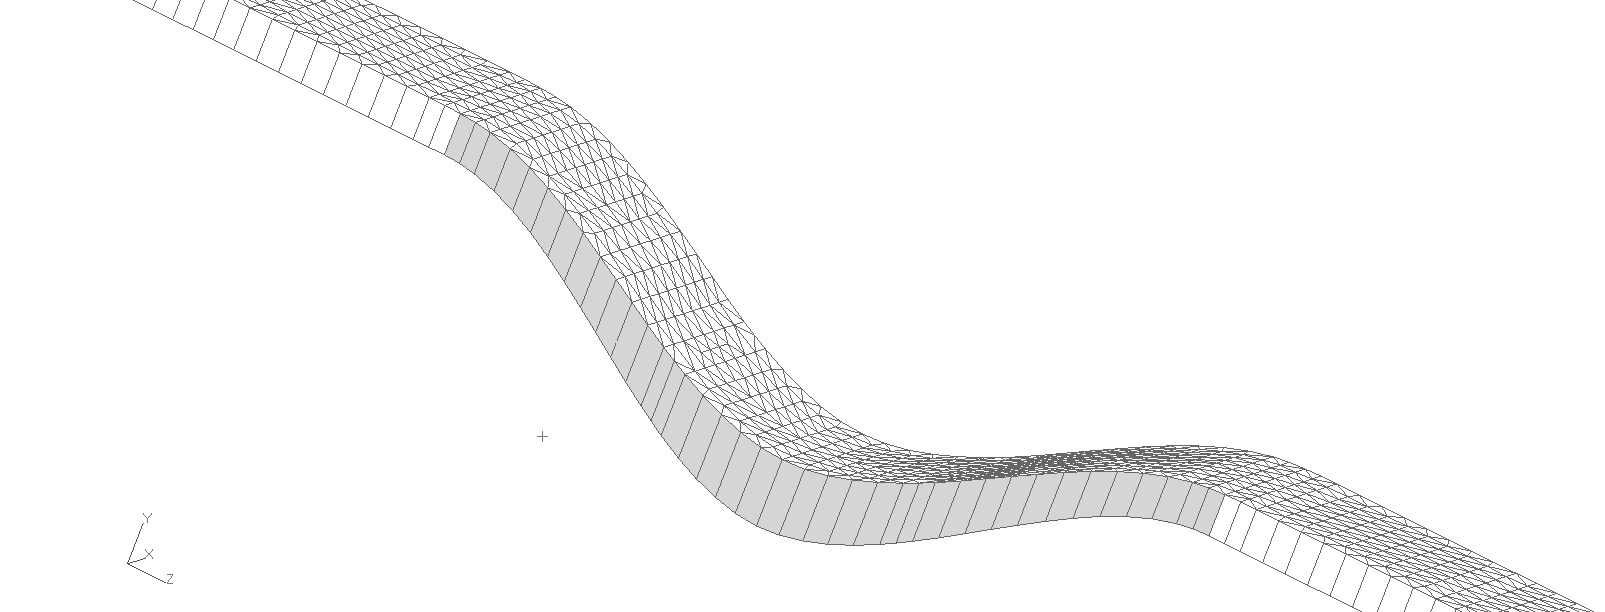
\includegraphics[width=0.9\textwidth]{simplifiedCentroplan}
\caption{Упрощенная модель центроплана с выделением исследуемой части}
\label{fig:CurvedKessonPatran}
\end{figure}

Использование в МКЭ-расчете такой упрощенной модели позволяет значительно ускорить процесс прочностного параметрического анализа при тех же вычислительных мощностях. Так, в упрощенной модели используется $\approx10000$ конечных элементов, в то время как в полной модели самолета используется $\approx270000$ конечных элементов.

Как было сказано выше, рассматриваемая модель имеет два варьируемых параметра: относительная координата нижней точки сечения и строительная высота сечения в плоскости XY в плоскости симметрии самолета. В качестве кривых, описывающих нижнюю и верхнюю поверхность кессона выбраны кубические сплайны, построенные через найденные исходя из выбранных параметров точки. Производные сплайнов в точках стыка фюзеляжа с крылом ($z=2.45\text{м}$) и в плоскости симметрии самолета ($z=0\text{м}$) приняты равными нулю. Пример модельного сечения центроплана в плоскости YZ приведен на Рис.\ref{fig:KessSectionExample}.

\begin{figure}[ht]
\centering
%\def\svgwidth{1\textwidth}
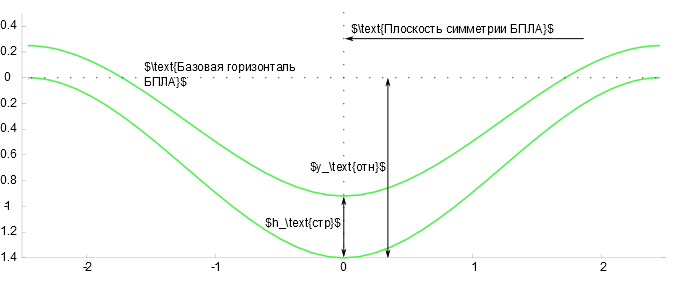
\includegraphics[width=1\textwidth]{KessSectionExample}
%\input{figures/KessSectionExample.pdf_tex}
\caption{Пример модельного поперечного сечения центроплана}
\label{fig:KessSectionExample}
\end{figure}


Выбор такой параметрической модели позволит в дальнейшем (вне рамок данной работы) включить в процесс оптимизации сечения также расчет аэродинамических нагрузок, что позволит полностью автоматизировать процесс оптимизации формы центроплана для центропланов такого типа. 

